% introduction
\begin{frame}{Beamer}

    \begin{itemize}
        \item A beamer is one of the 10 \LaTeX  document classes.
        \item Beamer is used heavily for making great looking and standardized
            presentations.
        \item \LaTeX has built-in themes (not templates) Eg: CambridgeUS theme
        \item They can be simple like this one, but are also highly customizable
            like the one shown below
        \item The best part is, they are in PDF format.
    \end{itemize}

    \center
    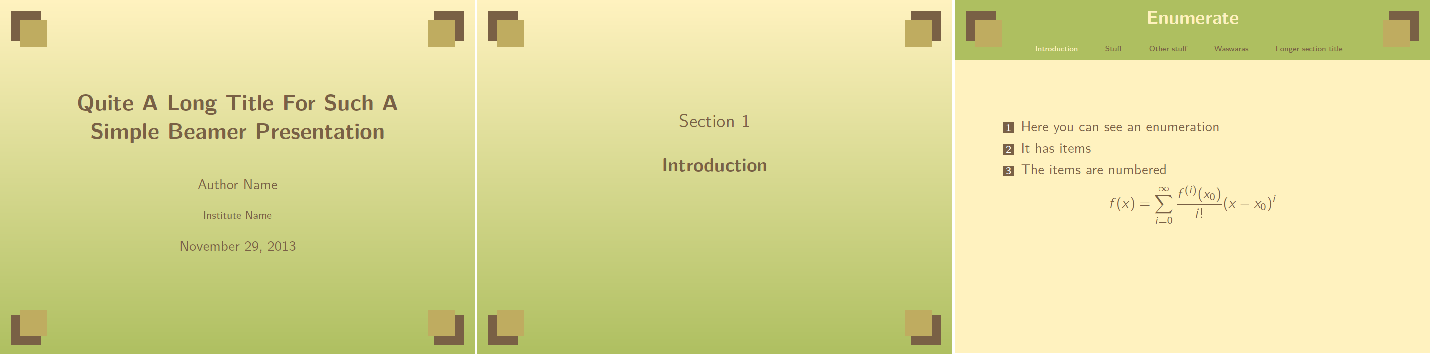
\includegraphics[width=\textwidth]{ugly.png}

\end{frame}


% beamer syntax
\begin{frame}{Beamer}{Make a basic Beamer}
    A "frame" in a beamer is what can be refered to as a slide in
    presentation.\vspace{1em}

    You can break a single frame into multiple pages by using the \texttt{\\pause}
    command. For example below itemization will load in multiple slides: \vspace{1em}

    \begin{enumerate}
        \item \pause this is first
        \item \pause this is second
        \item \pause this is third
    \end{enumerate}

    \pause
    Note:
    \begin{itemize}
        \item "Slide" in beamer unintuitively means, a page of a PDF file.
        \item Most themes also come with Navbar, at the bottom.
        \item Some usefull documentation can be found in
            \href{https://latex-beamer.com}{latex-beamer.com}
    \end{itemize}
\end{frame}

\begin{frame}{Beamer}{Overlays}
    Like pause, there are various different overlays to fit the needs.
    You can use the \texttt{onslide<n-m>} command to explicitly state the slide
    number in which an item appears in.\vspace{1em}

    Here's a demonstration of commands like  \texttt{onslide<n-m>},
    \texttt{only<n>} and \texttt{alt<n>}. \vspace{1em}

    \alt<6>{We are on slide 6}{We are not on slide 6 btw}
    \begin{enumerate}
        \onslide<2-6> \item this is second slide
        \onslide<4-6> \item this is fourth slide
        \onslide<3-6> \item this is third slide
        \only<5>{\item this only appears in 5th slide}
    \end{enumerate}
\end{frame}

% Blocks in beamer
\begin{frame}{Beamer}{Blocks in Beamer}
    \small
    Sometimes we need to display some information that convey some special
    messages. As an example, an information box with a title and some
    background color can deliver an important scientific fact. \vspace{1em}

    Here are some useful blocks: \pause
    \begin{block}{Custom block message}
        some content
    \end{block}
    \pause
    \begin{alertblock}{Custom alert message}
        some alert
    \end{alertblock}
    \pause
    \begin{exampleblock}{Custom example: 1.1}
        some example
    \end{exampleblock}
    \pause
    \footnotesize
    Making a some standard blocks, such as \texttt{proof}, \texttt{example}
    can be as easy as making environments. Using above custom block messages,
    it is also really easy to make your own environments.

\end{frame}


% Task
\begin{frame}{Beamer}{Task-1}
    Try solving the task-1.
\end{frame}
